% 
% Annual Cognitive Science Conference
% Sample LaTeX Paper -- Proceedings Format
% 

%% Change "letterpaper" in the following line to "a4paper"e if you must.

\documentclass[10pt,letterpaper]{article}

\usepackage{cogsci}
% Recommended, but optional, packages for figures and better typesetting:
\usepackage[margin=1in]{geometry} 
\usepackage{microtype}
\usepackage{graphicx}
\usepackage{subfigure}
\usepackage{booktabs} % for professional tables
\usepackage{nicefrac}       % compact symbols for 1/2f, etc.
\usepackage{microtype}      % microtypography
\usepackage{float}
\usepackage[colorlinks,allcolors=purple]{hyperref}
\usepackage{algorithm}
\usepackage{amsmath}
\usepackage{graphicx}
\usepackage[table,xcdraw]{xcolor}
\usepackage{gensymb}
\usepackage{stmaryrd}
\usepackage{amssymb}
\usepackage{todonotes}

%\cogscifinalcopy % Uncomment this line for the final submission 


\usepackage{pslatex}
\usepackage{apacite}


%\usepackage[none]{hyphenat} % Sometimes it can be useful to turn off
%hyphenation for purposes such as spell checking of the resulting
%PDF.  Uncomment this block to turn off hyphenation.


%\setlength\titlebox{4.5cm}
% You can expand the titlebox if you need extra space
% to show all the authors. Please do not make the titlebox
% smaller than 4.5cm (the original size).
%%If you do, we reserve the right to require you to change it back in
%%the camera-ready version, which could interfere with the timely
%%appearance of your paper in the Proceedings.



% \title{Contextually-adapted abstractions explain \\ contextually-adapted abstraction in language} 
\title{Discovering concept libraries through communication about object structure}
 
\author{{\large \bf Morton Ann Gernsbacher (MAG@Macc.Wisc.Edu)} \\
  Department of Psychology, 1202 W. Johnson Street \\
  Madison, WI 53706 USA
  \AND {\large \bf Sharon J.~Derry (SDJ@Macc.Wisc.Edu)} \\
  Department of Educational Psychology, 1025 W. Johnson Street \\
  Madison, WI 53706 USA}


\begin{document}

\maketitle


\begin{abstract}
% [SCRATCH] A crucial dimension in communication is the level of abstraction at which people pitch their language.
% While we do flexibly shift our words to suit the needs of different contexts, the ways in which we do so when describing compositional phenomena is less well understood.
% In this paper we present a novel set of hierarchical stimuli, and present an experiment in which we elicited compositional descriptions of these stimuli in different contexts. 
% We compare participants' descriptions to \textit{a priori} and learned measures of the formal structure of these stimuli, allowing us to assess the extent to which context shifts the level of abstraction reflected in participants' words.

\textbf{Keywords:} TBD
\end{abstract}


\section{Introduction} \label{sec-introduction}
% \textit{[CW: I will probably get to a major rewrite of this intro on *Saturday*. But earmarking that the main changes I'm *planning to make are*: to present the novel part of our work (with respect to the earlier work) as identifying the *vocabularies* people use across domains, rather than the individual words they use in free-naming tasks. that are characteristic of the basic level; in that way, what we have here is really a generalization of this notion of a default level of abstraction, extended to whole vocabularies used to discuss domains of complex scenes; and an information-theoretic hypothesis about DSL size + program length that we correlate with natural language vocabularies in Part II and Part III.]}

%% CW: jefan notes: rather than hypothesizing the basic level, i think it will be  more impactful to pose the theoretical question about representation-for-communication -- and reveal it through our library identification method, and discuss the basic-level thought as an implication at the end of the paper.
% RUNNING EXAMPLE: TBD? Needs to be some real world constructive task. 

% Examples of natural language communication of things with structure abound: | How to build a bike | How to build a house - windows, a door, |  ----We have specialized ways of talking about how to build a bike; your car; of a kitchen applicance; when we talk procedural tasks: furniture; people know about specialized words for recipes; ___; and for building architecture.\

%% 0: THE PHENOMENON: How do we talk about structure in the world? Give examples of talking about structure. 
%% 1: LITERATURE 1 Perceptual organization & visual concepts -- MEANINGS that carve up structure of the world.
%% the good: tradition of configural processing for many visual domains (objects; Biederman/Hummel; scenes: Melissa Vo)
%% the gap: a focus on holistic discrimination judgments rather than part structure -- % BUT: Most of this has been discrimination and labeling tasks. Not about structure; in complex scenes. -- and these have been point instance for instance-level language.
%% 2: LITERATURE 2 Constraints on communication -- LANGUEG / VOCABULARIES that carve the world.
%% the good: why do we have the vocabularies we do; and what are they bound to? the notion of negotiating a tradeoff between compression & expressivity %% \cite{kirby2015compression}, and many others.
%% the gap: those studies have been using artificial language (artificial tokens). small stimulus sets that don't vary that much in complexity and type. Really important limitations if we want to explain HOW people talk about structure. [Some of this is also less about structure (eg. color naming); others more about language evolution. But similar points about library size and compression.] -- and these have been point language for instance-level language.

%% 3: WHAT WE DID ABOUT IT: Formal link using program representations & library identification -- representational AND measurement innovations.)
    % WE propose a generic way of representing concepts (PROGRAMS)
%%  And: a linking function between program concepts to to REAL language. across broader variation in stimulus type & complexity. 
%%  what we learned and why LIT1 and LIT2 are both better off for it: perception people get structure; language people get where lexica come from (they carve at the joints of mental representations using this generic representational framework.) -- and this is a generic framework for doing this (exposing these information theoretic ideas)  AT SCALE for COMPLEX domains of stimuli. 
% Some nested clause mentioning: Ellis (?); Tian et. al; McCarthy et. al

% Our main contributions:
% LIT 1: A generic framework for discovering conceptual structure; our hypothesis space is over libraries. 
% LIT 2: Attempts to understand languages that emerge in iterated paradigms have been in restricted domains with low-stimulus variaiton and low-linguistic naturalism.
% People seem to communicate about structure. But how do we know what structure people actually represent? (Here, we have MUlTIPLE libraries that represent alternate hypotheses about structure -- what is the concept library people are actually using?) Prior work has evaluated SPECIFIC libraries.
% People seem to communicate this IN language. (This is a particularly good window into the mind of their thoughts about structure.) We ALSO have a library identification tool that tells you which ONES best fit their overt behavior in language.

%%%% PHENOMENON: How do we talk about structure in the world? 
The world is filled with a great variety of objects, yet people have no trouble finding ways to communicate about them. 
People not only know what to call a given object, but also how to describe its structure --- what it is made of and how those parts are arranged.
In other words, the underlying structure of our percepts and concepts is often reflected in the words of our language.
For example, a car has a \emph{body}, \emph{windows}, \emph{doors}, and \emph{wheels}.
Houses also have \emph{doors} and \emph{windows} (even if they look different from those of cars), but may be multiple \emph{stories} and have \emph{pillars} or \emph{porches}.
Even for an object someone has never seen before, such as a new building or device, people can generally figure out how to describe it so that they are understood \cite{hawkins2020characterizing}. 
What are the computational mechanisms that enable people to so robustly communicate their understanding of how the world is organized?

%%%% PERCEPTION
On one hand, the ability to parse the visual world into meaningful units is central to theories of perceptual organization
\cite{hoffman1984parts,biederman1987recognition,palmer1977hierarchical,tversky1984objects}.
\cite{rosch1976basic}

%%%% COMMUNICATION
People choose flexibly between different levels of abstraction and specificity in language -- we might switch between referring to our \textit{car} to distinguish it from other modes of transportation, and referring to our \textit{orange minivan} to pick it out from other models at a parking lot.
Classical theories have suggested that people consider co-occurring attributes of objects \shortcite{tversky1984objects}, such as their function, and suggest a characteristic ``elbow curve" that trades off between the informativeness of any one attribute and its discriminability with respect to a full domain. Later work has focused on the importance of object \textit{parts} in determining the basic level, both for familiar objects (a \textit{chair} might have \textit{legs}, \textit{arms}, and a \textit{seat}); and for simple artificial, compositional stimuli (an image made of \textit{wavy lines} and \textit{polka dots}) \shortcite{murphy1991parts, palmer1977hierarchical}. But how do people determine \textit{which} set of part concepts to use in context?

Consider, for example, the drawing of the object at the top of Fig. \ref{fig:task}B, or the block tower at the bottom. Each can be described using language that picks out sets of parts at different levels of abstraction. How should a speaker choose between describing the drawing using a simple, but low-level vocabulary of a few basic shapes (like \textit{lines, circles}, and \textit{squares}) instead of names for its higher-order parts (like an \textit{antenna} or \textit{dial}, or even \textit{a row of dials}); or between describing the block tower by naming individual \textit{red block} and \textit{blue blocks}, as opposed to higher-level abstractions like a \textit{roof} and \textit{floors}? What determines the basic level of abstraction a person chooses to describe these compositional stimuli, amongst the possible vocabularies of nameable parts?

%%%% PROGRAM-LIKE CONCEPTS
We approach this question through a formal computational model that builds on two related lines of work. Prior word learning models \shortcite{xu2007word,frank2009using} have proposed that for \textit{individual} category names, contextual word choice can be modeled as Bayesian optimality over a hypothesis space of alternatives. In tandem, recent work has proposed \textit{program learning} as a powerful formal model for the underlying conceptual representations of objects, building on classic notions of a compositional mental \textit{language of thought} \shortcite{lake2015human,ellis2020dreamcoder}. Under this modeling approach, concepts are represented as structured \textit{programs} written in  domain-specific languages (DSLs) of compositional concept primitives. Agents may build on an initial library of primitive concepts with new \textit{abstractions}, chunked sub-routines which abstract over programs written in lower-level primitives. Prior experimental work has used models of program \textit{abstraction} learning to explain people's motor abstraction learning over domains of compositional drawing stimuli \shortcite{tian2020learning}; and to model human coordination on shared object representations when assembling simple, compositional block towers \shortcite{mccarthy2021learning}.


%%%% FRAMEWORK TO INFER CONCEPT LIBRARY PEOPLE USING TO COMMUNICATE





\begin{figure*}[h]
  \begin{center}
  \includegraphics[width=0.99\linewidth]{figures/lax_task.pdf}
  \caption{A) We designed two domains that hierarchically decomposed into 4 subdomains, each containing different distributions of compositional parts over the same base primitives (basic shapes or blocks). B) Participants wrote instructions for generating a set of stimuli from a single domain, in sequences of `what'-`where' steps.}
  \label{fig:task}
  \end{center}
 \end{figure*}

Here, we suggest that the \textit{level of abstraction} people choose when describing a domain of related, compositional objects -- like the \textit{technical drawings} and \textit{block towers} in Fig. \ref{fig:task}A -- can be modeled as a \textit{DSL choice} over possible libraries of formal conceptual primitives at differing levels of abstraction, which can be composed into generative programs to produce any chosen object. We hypothesize that the level of abstraction reflects a contextual tradeoff between \textbf{DSL size} (the total number of concepts necessary to represent objects in a given domain, using a particular set of conceptual primitives) and \textbf{program description length} (how many primitives in the chosen DSL must be composed to describe any individual item drawn from the domain). This hypothesis formalizes an intuitive tradeoff in classical, part-based theories of the basic level: a low-level set of parts (like describing the drawing in terms of \textit{squares} and \textit{circles}) uses a small vocabulary, but requires  many words to describe an individual object; a high-level but specific set of parts (one with specialized terms for different makes and models of dressers, for instance) might succinctly describe any one object, but at the expense of requiring a large overall vocabulary to describe a diverse domain.

To evaluate this, we develop a dataset of two domains of hierarchical object stimuli (Fig. \ref{fig:task}A), and conduct a procedural language experiment to elicit human descriptions of each object. We find that people use different, context-specific linguistic vocabularies dependent on the subdomain of objects (Part I). We then introduce the formal representational approach, defining program \textit{DSLs} at varying levels of abstraction, that we use to model abstraction choice in language. Using this, we first use \textit{program description length} alone to correlate programs and language (Part II), and discuss findings and challenges of this approach. Finally, we introduce a more expressive \textit{program-language alignment} model, and find that people's language is best explained in this model by DSLs that jointly minimize program description length \textit{and} overall DSL size (Part III).

\section{Part I: Descriptions are sensitive to object structure} \label{sec-part-i}
% Consider how you might describe the drawing or block tower in Figure \ref{fig:task}A. Both images could be described in language that carves up the image, intuitively, at multiple levels of abstraction -- how would you choose between describing the drawing using a simple but low-level vocabulary of basic strokes (like \textit{lines, circles, and squares}) vs. a set of names for some of its functional parts (like \textit{antenna} or \textit{dial}); or between describing the block tower as composed of \textit{red blocks} and \textit{blue blocks} vs. of higher-level parts like a \textit{roof} and \textit{floors}?

% 
\todo{Introduce this section}
% Why design these stimuli? Why run an experiment?

% All we know about this dataset is that it has STRUCTURE; what we expose is variation in nameability. 

% Created a set of stimuli with variation in structure 
% Extend from holistic judgements and labeling to more detailed descriptions of object structure.

% lots of parts
% lots of structure

\subsection{Methods}

\paragraph{Participants}
465 participants recruited from Prolific completed the task. 
Participants provided informed consent and were paid approximately \$15 per hour for their time.

\paragraph{Stimuli} 

% todo: tie to program abstraction
% Desiderata: 1) varied set of categories, 2) hierarchical structure; 3) primitives + higher-order abstractions available to describe, 4) novel + evocative
% 	What do these buy us?
% #1 more general findings
% #2 reminiscent of hierarchical structure of real-world concepts
% #3 allows us to test the notion of "basic-level" but for parts (Rosch et al.) (“just right” level of abstraction)
% #4 lets us look at learning (later)

% To accomplish this, we constructed two domains of stimuli-- (\textit{technical drawings} and \textit{block towers}) (Fig. \ref{fig:task}A)-- that are each generated from a shared base set of procedural, symbolic primitives (shapes or blocks).
% We then ran an experiment to elicit language from subjects who were familiarized with stimuli from a specific \textit{subdomain}-- each containing items generated from distinct generating procedures over these primitives and varying hierarchically in terms of their compositional parts.
% We hypothesized that the vocabularies people used to describe each stimulus would be \textit{context-specific}: that participants would tend to use different vocabularies tailored to the subdomain distribution of stimuli they were shown.

\begin{figure}
  \begin{center}
  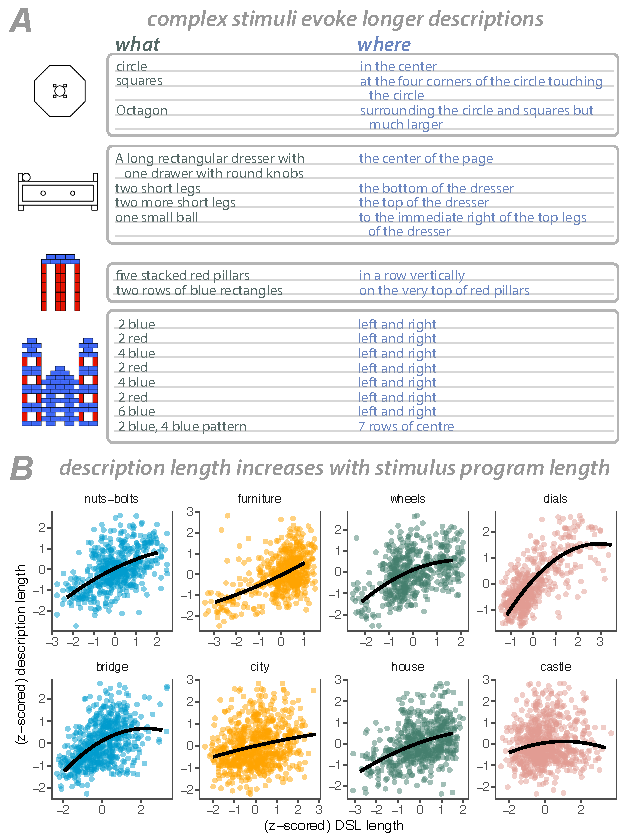
\includegraphics[width=0.99\linewidth]{figures/lax_description_length.pdf}
  \caption{Example descriptions suggest that more complex stimuli evoke longer descriptions (A), which is also supported by a comparison of description length with the length of the program used to generate each image (B). Quadratic line of best fit shown. }
  \label{fig:words}
  \end{center}
\end{figure}


% different motivation for artificial stimuli: XXX
% Don't need to talk about nameability: say it has structure
% We expose variability in structure (x-axis in part II)
% While many such categories exist in the real world, these often come with canonical ways of being decomposed into parts, or have a hierarchical structure that is too ambiguous to permit the formal modeling approach of \ref{sec-part-ii}.

As a core goal of this project was to evaluate whether the language used to describe the \textit{compositional structure} of an object is affected by context, we needed a set of stimuli that a) had varied compositional structure, and b) could be divided into multiple distinct categories. 
% To construct a set of stimuli with variation in compositional structure, 
We procedurally generated stimuli using a set of nested, parametric functions operating on a set of base primitives, hierarchically composing them into increasingly complex, recursively-defined parts.
A \textit{dresser}, for example, is composed of \textit{drawers}, which are in turn composed of a \textit{panel} and \textit{knobs}, and which are defined finally over a shared set of simple shape primitives (Fig. \ref{fig:task}B).

Our stimulus set was divided into two distinct \textit{domains}, each procedurally generated from a different set of base primitives:
\textit{technical drawings} were designed to resemble technical drawings of functional objects, and were composed of simple geometric shapes; 
\textit{block towers} were designed to resemble simple architectural models, and were composed of 2D rectangular blocks.
% Different compositional structure within domain (difference between subdomains)
Each \textit{domain} was further divided into four \textit{subdomains}, each defined by a distinct generative procedure that was hand-designed to produce objects of a recognizable subordinate category (e.g. \textit{furniture}, \textit{castle}) from a set of predefined abstractions (e.g. \textit{legs}, \textit{tower}).
We enumerated all possible stimuli for each subdomain, and selected a random but biased sample of each to obtain 250 stimuli of varying complexity for each subdomain, along with corresponding programs expressed in a base DSL.

\paragraph{Task procedure}

Participant produced descriptions for 10 items from a single \textit{subdomain} (e.g. only \textit{castles}). 
To familiarize participants with the task-relevant distribution of stimuli and part abstractions, participants first clicked through 25 images of other stimuli from their subdomain. 
As participants typed descriptions, they also saw previews for 7 upcoming stimuli.
% However participants were not encouraged to produce instructions that disambiguated their items from others in their domain, as in a traditional reference game.
To evoke a thorough description of each object's component parts, we asked participants to type a complete ``step-by-step'' procedure for reconstructing a stimulus, either describing how to ``draw'' the item if it was a \textit{technical drawing}, or how to ``build'' the item if it was a \textit{block tower}.
To disentangle the language used to refer to the parts of an object from spatial descriptions of where those parts should go, participants typed their responses, step-by-step, into a pair of \textit{what} and \textit{where} text boxes (Fig. \ref{fig:task}B), describing in each step what should be drawn/placed where to reproduce the target image.
Participants could add as many instruction steps as they liked for each stimulus, and had no time limit.



\paragraph{Language preprocessing} % spacy, en_core_web_lg,
To better investigate the content of the instructions generated by participants, we use the spaCy NLP library to extract and lemmatize words, using part-of-speech (POS) tagging to remove determiners and punctuation. We also replaced high-frequency typos (``sqaure,'' ``cirlce,'' etc.) and spelling variations (``centre,'' ``colour,'' etc.) with their canonical spellings in US English.

\subsection{Results}
% ($b=XXX$, $t=XXX$, $p=XXX$)
% $XXX\%$ (95\% CI: $[XXX, XXX]$)

\paragraph{Participants produced longer descriptions for block tower stimuli}

\todo{Qualitative observation that more complex structures look like they result in longer descriptions.}
(Fig. \ref{fig:words}A)

To assess how participants' language differed across the two domains, we ran a linear mixed effects models with fixed effects for domain and trial number, an interaction term between the two, as well as random intercepts for subdomain and participant.
\textit{Block tower} descriptions tended to be longer than those for \textit{technical drawings}, both in terms of the number of \textit{what-where} steps provided ($b=5.08$, $t=10.9$, $p<0.001$) and raw character counts ($b=373$, $t=8.24$, $p<0.001$).
We suspected that participants identified more entities in the \textit{block tower} stimuli, which was supported by a greater number of words entered in the \textit{what} boxes of \textit{block towers} than for \textit{technical drawings} ($b=25.8$, $t=9.55$, $p<0.001$).
In all of the above models, we found a significant negative fixed effect of trial number, as well as an interaction between trial number and domain consistent with a faster drop off in description length for block towers.
This suggests that participants produced more concise instructions over time, consistent with prior work suggesting a shift to higher-level abstractions as people repeatedly describe block towers \cite{mccarthy2021learning}. % is this point too misleading/ distracting?

% Nevertheless, it appeared that instructions produced for both domains spanned a range of levels of abstraction (Fig. \ref{fig:words} A), with some referring to lower level primitives (i.e. geometric shapes and individual blocks) and some to more abstract compositions of these lower elements (e.g. ``desks'', ``pillars'', and ``castle-like block towers'').
% Stimuli from each domain were constructed from distinct sets of base primitives that can be combined according to distinct sets of constraints, allowing us to investigate whether participants systematically varied their vocabulary according to their context.


% n_steps ~ domain * trial_num + (1 | subdomain) + (1 | gameID)
%                              Estimate Std. Error         df t value Pr(>|t|)    
% (Intercept)                   4.36409    0.33821    8.47840  12.904 7.25e-07 ***
% domainstructures              5.07991    0.46552    7.58715  10.912 6.61e-06 ***
% trial_num                    -0.06105    0.02143 4183.00156  -2.848  0.00442 ** 
% domainstructures:trial_num   -0.29242    0.02878 4183.00156 -10.162  < 2e-16 ***


% char_sum ~ domain * trial_num + (1 | subdomain) + (1 | gameID)
% Fixed effects:
%                           Estimate Std. Error       df t value Pr(>|t|)    
% (Intercept)                 305.566     32.635    7.475   9.363 2.16e-05 ***
% domainstructures            373.091     45.288    6.922   8.238 8.04e-05 ***
% trial_num                    -5.493      1.640 4182.994  -3.350 0.000817 ***
% domainstructures:trial_num  -29.624      2.201 4182.994 -13.457  < 2e-16 ***


% n_whats_filtered ~ domain * trial_num + (1 | subdomain) + (1 |      gameID)
%                             Estimate Std. Error        df t value Pr(>|t|)    
% (Intercept)                  17.6224     1.9618    7.9137   8.983 2.01e-05 ***
% domainstructures             25.8495     2.7060    7.1447   9.553 2.53e-05 ***
% trial_num                    -0.2667     0.1174 4182.9953  -2.272   0.0231 *  
% domainstructures:trial_num   -1.5601     0.1576 4182.9953  -9.900  < 2e-16 ***


% Instructions produced for each of the two domains differed in several dimensions.
% \textit{Block tower} instructions tended to be longer than those for \textit{technical drawings}, both in terms of the number of instruction steps provided ($t=-27.8$, $p<0.001$) and the raw character counts ($t=-20.3$, $p<0.001$).
% using normal t-tests for these. Data aren't necessarily normally distributed though.
% n-steps t-test
% Ttest_indResult(statistic=-27.765628342013194, pvalue=4.004442116161361e-157)
%
% character count t-test
% Ttest_indResult(statistic=-20.30653751103832, pvalue=6.629047614713647e-88)
%
% What words
% Ttest_indResult(statistic=-24.778853065643887, pvalue=2.030452944756843e-127)
%
% 

\paragraph{Correlating language length with program description length}
% Are people sensitive to the structure within a subdomain?
% \cite{sun2021seeing}: the correlation of \textit{program description length} to \textit{language description length}.
% Evaluating the simplest possible relationship between natural-language descriptions and formal programs: do people tend to use more words to describe more complex objects? 
\todo{link from prev section}
For each object, we operationalized natural-language description length using the mean number of words entered in the \textit{what} text boxes and operationalized the program length as the number of tokens required to express that object in the given DSL.
To control for clustered participant-level variation in the use of the text boxes, we constructed a mixed-effects model predicting the length of each natural-language description. 
We included fixed effects of the object's subdomain (with eight levels) and the corresponding program length in the DSL, with random intercepts and effects of program length at the participant-level. 
For the base DSL, we observed a significant main effect of program length, $t(318)=14.8, p < 0.001$ across all subdomains (Fig.~\ref{fig:libraries_correlations}B).
We also found that a model including an additional quadratic effect of program length, allowing for a non-linear relationship, significantly improved the fit, $\chi^2(3)=38.6$, although these relationships varied somewhat across subdomains.
\todo{Explain challenges with using this approach.}
% Holistic- doesn't look at the structure of the stimuli, disregards meaning of words

\begin{figure*}
  \begin{center}
  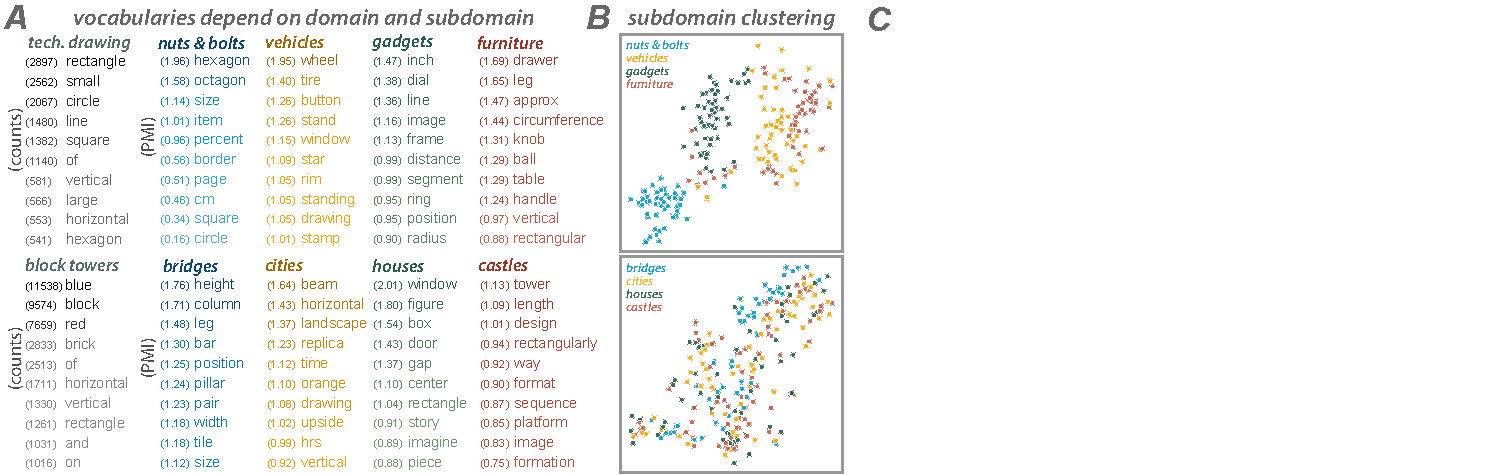
\includegraphics[width=0.98\linewidth]{figures/lax_vocabularies.pdf}
  \caption{A) XXX B) Word counts for domain. PMI for subdomains. C) Clustering of word-count vectors shows more distinct language across subdomains of technical drawings than of block towers. Each point is a participant, each of whom described items in a single subdomain. }
  \label{fig:libraries_correlations}
  \end{center}
  \end{figure*}

\section{FROM OLD PART II: Distribute across new parts I and II}

Prior work \shortcite{xu2007word} has demonstrated that a context-sensitive, ``basic level" for common noun choices can be modeled as an optimal choice from a \textit{hypothesis space} of alternatives, using a Bayesian model over object-kind categories. For this work, however, explaining language usage requires a hypothesis space which can scalably account for differing levels of abstraction in a complex space of compositional stimuli, and the extended, multi-word instructions generated in the procedural language task.

In this section, we introduce the formal representational approach we use to model levels of conceptual abstraction: a hypothesis space of related, recursively defined \textit{domain specific languages} (DSLs), containing \textit{program abstractions} of increasing complexity defined over the original base set of low-level primitives (Fig. \ref{fig:libraries_correlations} A). These DSLs formalize the relationship between subdomain-specific \textit{parts} used to generate individual stimuli. Program abstractions for higher order parts like a \textit{wheel} are formally defined over the lower-level base primitive \textit{strokes} that generate them. Given a particular DSL, the generating program for any given stimulus can be formally re-expressed at a given level of abstraction (the original generating program for a vehicle, initially written in terms of individual \textit{squares} and \textit{circles}, can be automatically rewritten in terms of higher order \textit{wheels} and \textit{base} program abstractions).

Given a hypothesis space of potential DSLs, how should we determine whether any one of them best explains human language? We begin in this section with a metric proposed in prior work \cite{sun2021seeing}: the correlation of \textit{program description length} to \textit{language description length}. We discuss formal challenges for this metric posed by a hypothesis space of DSLs at differing levels of abstraction, each of which can re-represent the generating program for any given stimulus.

\subsection{Methods}
\paragraph{Defining increasingly abstract DSLs} Prior work \shortcite{ellis2020dreamcoder,tian2020learning,mccarthy2021learning} has modeled human conceptual abstraction as iterative, context-dependent \textit{program abstraction}: starting from an initial DSL of program components, higher order DSLs can be defined by adding in chunked sub-routines, or program \textit{abstractions}, which build on the lower-level primitives. While we draw on this formal representational approach, we found in preliminary experiments that the automated DSL-learning procedures used in prior work do not scale well to the larger, more complex generative programs we consider here, and see automated DSL discovery as a promising avenue for future work.

Instead, here, we construct DSLs at increasing levels of abstraction using the ground truth generative model used to initially generate stimuli in each domain and subdomain. Specifically, we exploit the parametric structure of the procedural generative models described in Part I: stimuli are generated within each subdomain by enumerating over nested parametric subroutines of recursively defined parts, finally bottoming out in the shared base DSL for the domain (for instance, the \textit{furniture} stimuli are generated by composing primitive shapes in the base DSL to create \textit{knob} components, which are repeated and translated to create \textit{rows of knobs}, composed into \textit{drawers}, and then themselves translate into \textit{stacks of drawers}). Factoring these nested subroutines into program abstractions allows us to formally introduce new program components, and re-represent each stimulus in terms of these higher-order components, as in prior work.

For maximum discriminability between DSLs of differing levels of abstraction, and comparability across subdomains, we construct DSLs at three coarse grains of abstraction (see example components visualized from these DSLs for each subdomain in Fig.\ref{fig:libraries_correlations} A). We find that this yields distinct, interpretable libraries which formally re-represent each subdomain from components of increasing complexity. However, bucketizing these abstractions into three discrete levels (rather than incrementally considering DSLs which add all possible subroutines) does introduce some arbitrariness to the DSL construction, as we discuss; we see this as rich grounds for future work to scale the automated library learning procedures like that in \shortcite{ellis2020dreamcoder} (which introduces a formal Bayesian model to arbitrate amongst potential DSLs).
% We choose to consider the DSLs (and the rewritten stimulus programs under each DSL) both with and without the numeric parameters that vary across each subdomain (e.g. to enumerate dressers with \textit{two}, \textit{three}, and \textit{four} drawers); while they can be described in language, we expected that many numeric parameters would not be visually distinct (such as sizing parameters) or primarily responsible for variation in language. 
In total, for each subdomain, we considered the following DSLs, corresponding to coarsely-bucketed levels of abstraction:
\begin{itemize}
    \setlength\itemsep{0.1em}
    \item \textbf{Base DSL}: the low-level shared primitives (strokes and blocks) across the full domain.
    
    \item \textbf{$L_1$}: a  DSL corresponding to first-order parametric variation (eg. lines rotated into polygons; knobs composed of primitive shapes);
    
    \item \textbf{$L_2$}: a  DSL corresponding to intermediate parametric variation (eg. rows of knobs);
    
    \item \textbf{$L_3$}: a DSL corresponding to high-level parametric variation (dressers with varying numbers of drawers)
\end{itemize}

Fig. \ref{fig:libraries_correlations}A shows sample visualized components from each subdomain within each DSL, including the initial shared base DSL. We release the full generative procedure, parameterized abstraction generation, and individual DSLs and programs for each subdomain in the code repository.

%% we choose three coarse grains of abstraction. There is some arbitrariness to this choice, as we discuss in this and later sections. However, as seen in Fig X, this yields interpretable libraries which formally re-represent each program from generating components of increasing complexity.

% As described in Part I, stimuli in each subdomain are generated procedurally using nested levels of recursive, parametric variation: for instance, the \textit{dials} stimuli are generated first by nesting sets of primitive shapes in the base DSL to create \textit{dial} parts, which are themselves repeated and translated to create the \textit{rows of dials} in many of the images. Similarly, the \textit{house} stimuli are generated by first composing the blue and red block primitive shapes to create higher-order \textit{window} and \textit{brick} parts, which are tiled to create individual \textit{floors}, which are themselves stacked to create entire \textit{walls}. 

% Using the underlying procedural generative model for each subdomain, we therefore introduce contextual program abstractions into the base DSL -- and re-represent the generative program for each stimulus using these abstractions -- at three increasing levels of abstraction, corresponding to nested parametric variation over parts. These levels of abstraction, while driven by the underlying generative procedure, are chosen manually based on parametric depth -- clearly, there are more than three possible levels of variation in each domain. Future work can investigate additional possible levels of abstraction, as well as bottom-up methods for automatically discovering these abstractions and re-writing the generative programs from their base primitives (as in [CITE Ellis]).

% This parametric variation is context-specific, with increasing context-specificity at increasing levels of abstraction (Fig. \ref{fig:lanuage_libraries} A): for instance, in contrast to the \textit{dials} domain, for instance, base primitives in the \textit{furniture} domain are first used to generate individual \textit{handles, drawers, and legs}; then into \textit{rows of handles, stacks of drawers, and sets of legs}; and finally into entire  \textit{bookshelves} or \textit{lounges}.
 
 
% Restructure:
% How should we link DSLs to language?
% Prior work has tried this: (Sun and Firestone)
% Introduce more sophisticated DSLs
% Motivate Part III: using translation models (+ different measures from language length)

% Each stimulus in Sec. \ref{sec-part-i} can be represented with its generating program in a base DSL of low-level primitives (\textit{strokes} in technical drawings; \textit{blocks} in block towers) shared across the domain. Before considering more abstract representations, we can first ask: do these underlying program representations at all predict the language people use to describe each stimulus? We conduct a control experiment to establish an initial correspondence between the procedural program representations in the base DSL and human language, by correlating \textit{program description length} (program token counts) in the base DSL with \textit{language description length} (language token counts.)  

% We hypothesized a positive, but non-linear, correlation between description lengths in the base DSL and human language: we expect that even when measured in low-level primitives, more complex stimuli should require more words to describe; but we also expect that the existence of domain-specific abstractions named in language (as established in Section I) should mean that people's language length should not scale linearly with the number of blocks or strokes in each stimulus.


\section{Part II: Content of participants' language reflects compositional structure of objects}\label{sec-part-ii}
% \section{Part II: Aligning programs to language reveals DSLs that best explain language}\label{sec-part-ii}

\begin{figure}
  \begin{center}
  \includegraphics[width=0.98\linewidth]{figures/lax_libraries.pdf}
  \caption{A) }
  \label{fig:libraries_correlations}
  \end{center}
  \end{figure}

\begin{figure}[h]
  \begin{center}
  \includegraphics[width=\linewidth]{figures/fig_perplexity_costs_narrow.pdf}
  \caption{[SCRATCH] Perplexity (blue, left y-axis) and combined DSL size and program length (red, right y-axis) within each subdomain; shown with respect to DSL size; DSL size increases with additional higher-level abstractions. Shown for the base DSL, $L_1$, $L_2$, and $L_3$.}\label{fig:perplexity-length}
  \end{center}
\end{figure} 

The formal representational approach we introduce in Part II suggests an intriguing correlation between abstraction and description length. More abstract DSLs \textit{reduce} the description length of individual programs (the drawing program for a furniture stimulus, for instance, might shorten dramatically from a long sequence of individual shape primitives to one from a small number of higher-order \textit{drawers} and \textit{legs}). However, these new program abstractions increase the size of the DSL itself: more abstract DSLs contain more and increasingly specific components required to express the subdomain as a whole. In the limit, the most abstract DSL would contain a single subroutine for each distinct stimulus in the subdomain: allowing a maximally compact description of any one object, but at the expense of a DSL the size of the subdomain itself.

This observation follows from multiple related models in prior work. The automated Bayesian DSL learning models in \shortcite{ellis2020dreamcoder,tian2020learning} introduce an additional prior over DSL size; this prior is also similar to the hypothesis-space \textit{size principle} in the word learning model in \shortcite{xu2007word}. Information-theoretic models based on optimal coding theory also consider a related, extended notion of description length [CITE]: based on the description length of any one ‘message’ expressible in a given code, as well as the vocabulary size of the code over all.

Together, this prior work suggests a formal hypothesis about the basic level of abstraction: that people choose a level of abstraction in language corresponding to a set of concepts, (modeled a given DSL) which \textit{jointly} minimizes both the DSL size across the full domain and the expected description length of programs for individual stimuli.

To evaluate this hypothesis, however, Part II also motivated the need for richer models (beyond correlations in language and program length) for correlating programs in higher-order DSLs and language. Therefore, in this section we first introduce a \textit{program-language alignment model} based on statistical machine translation, which infers alignments between specific DSL components and tokens in human language. We show how this model can be used to measure fit between DSLs and language, and find that it indeed identifies DSLs which optimize for both program length and DSL size as those that best predict language usage from our task.


\subsection{Methods}
\paragraph{Program-language alignment model}
Part II attempted to measure correspondences between programs and language using a simple description length correlation metric. As discussed, however, this metric ignores token identity in language and programs. We are interested in correlating specific components within a DSL with words in language. Therefore, we introduce a \textit{program-language alignment} model based on statistical machine translation models, which infers alignments between tokens in programs and language, and defines a formal likelihood of observed language given any one program.

We use the IBM Model 1 \shortcite{gal2013systematic} statistical translation model, which has a simple but interpretable formulation that we found to be effective for our setting. This model infers explicit, token-token alignments from a training corpus of paired programs and language for each stimulus. It does not consider token order, and estimates a predictive likelihood $P(language | program)$ decomposed as an independent product of token-token translation likelihoods, $\Pi P(l | p)$, between aligned words $l$ and program components $p$. Following standards in the translation literature, we evaluate \textit{mean log-likelihood} (mean across predicted word tokens) [CITE] under the fit model, which measures average word-predictability given a source program and controls for sentence length (this metric also corresponds monotonically to \textit{negative perplexity}).

We evaluate each DSL $L_i$ for each subdomain using a cross-validated evaluation scheme (using heldout batches of n=5 stimulus), fitting the model to all pairs of training programs (re-expressed under the DSL) and language for each stimulus and then evaluating the model on the heldout stimuli. For comparison with Part II, we consider only the pre-processed `what' descriptions for each stimulus. 

\subsection{Results}

%%% Looking at content rather than length

\paragraph{Vocabularies are sensitive to domain and subdomain contexts}

\todo{Make more general points (while referencing fig 2A) that set up later analyses}
We suspected that the distinct sets of base primitives comprising objects in either domain would be reflected in a difference in the vocabularies used in participants' descriptions.
Fig. \ref{fig:words} B (left column) shows the most common words used in each domain (\textit{what} boxes only).
We see that for \textit{technical drawings} these include basic shapes (``rectangle'',``circle'',``line''), whereas for \textit{block towers} they refer to blocks (``block'',``brick'',``red'', ``blue'').

Each of the four subdomains of \textit{technical drawings} and \textit{block towers} contained a unique distribution of procedural abstractions.
% The distribution of procedural abstractions across the stimuli was particular to each of the the four subdomains of \textit{technical drawings} and \textit{block towers}.
Did participants' language also reflect these finer-grained differences?
% Participants' instructions reflected abstractions that were unique to the four subdomains of \textit{technical drawings} and \textit{block towers}, respectively. 
To quantify which words were most characteristic of each subdomain, we computed the pointwise mutual information (PMI, Eq.~\ref{eq:pmi}) of each word with respect to the four subdomains. 
Intuitively, PMI favors words that occur frequently in a subdomain (numerator), controlling for both the overall prevalence of the word and the relative amount of data for each subdomain (denominator). In our case, the distribution of examples in each subdomain $p(\mathcal{D}_{sub}) \approx \frac{1}{4}$ was approximately uniform.

To correct for bias towards low-frequency words, we applied Laplace smoothing with $\alpha=1/|\mathcal{V}_\mathcal{D}|$ pseudocounts, where $\mathcal{V}_\mathcal{D}$ is the vocabulary of all unique words in the domain. 
In constructing $\mathcal{V}_\mathcal{D}$, we included only noun words (as identified by POS tagging) from the \textit{what} fields that occurred at least $n=5$ times in the dataset. The PMI values for words in \textit{technical drawings} and \textit{block towers} were computed independently.

\begin{equation} \label{eq:pmi}
PMI = \log \dfrac{p(w, \mathcal{D}_{sub})}{p(w)p(\mathcal{D}_{sub})}
\end{equation}

Words referring to the base primitives shared across subdomains, which were among the most frequently occurring in each domain, were generally not among the top-PMI words for the subdomains, as predicted.
Consistent with the design principles of our dataset, many of the top-PMI words corresponded to mid-level abstractions referring to nameable object parts (Fig. \ref{fig:words}B). 
For instance, in \textit{furniture}, participants used words like ``drawer,'' and ``leg''; in \textit{vehicles}, they used ``wheel,'' and ``tire''; and in \textit{houses}, they used ``window,'' and ``door.''
Abstractions referring to high-level object categories were occasionally present for some subdomains (e.g., ``table,'' ``tower,'' ``landscape''); notably, however, participants did not generally include category-level words like ``vehicle,'' ``castle,'' ``city,'' or ``house'' in their instructions.

% F-statistic
To quantitatively assess whether participants used different distributions of words for each subdomain, we calculated an F-statistic, separately for each domain, to measure how well the assignment of trials to subdomains explained variance in word count vectors (F-statistic, Eq.~\ref{eq:f}).
\begin{equation} \label{eq:f}
F = \dfrac{between\, group\, variability}{within\, group\, variability}
\end{equation}
We compared this value to a baseline calculated from random assignments of trials to 4 groups, to determine whether the words used within a subdomain explained more variance in word counts.
We found that this was the case for \textit{technical drawings}: ($\Delta F = 10.5$, 95\% CI: [$9.87$, $11.0$], $p=0$), confirming that participants' vocabularies did differ depending on their subdomain context. %need to be careful about phrasing here
For \textit{block towers}, however, this difference was marginally significant $\Delta F = 1.24$, 95\% CI: [$0.234$, $1.96$], $p=0.054$, suggesting that participants used less distinct language across the different subdomains of \textit{block towers}.
This suggestion was also borne out by visualizations of participants' vocabularies (Fig. \ref{fig:words}C).
We counted the occurrences of each word across all of a participants' trials, computed the 30 principle components of these counts using PCA, and visualized t-SNE embeddings of these components.
While participants' vocabularies for \textit{technical drawings} are largely separable by subdomain, those for \textit{block towers} are more interspersed.
It appears that, compared to the subdomains of \textit{technical drawings}, \textit{block towers} subdomains elicit less distinct sets of descriptors, which could be due to the mid-level abstractions being less nameable than those of \textit{technical drawings}, or to them being less perceptually identifiable. % and a higher reliance on base primitives?


\subsection{[CHANGE] Library correlations}

Fig. \ref{fig:libraries_correlations} (blue) shows cross-validated \textit{mean log-likelihoods} for heldout stimuli, plotted with respect to $log(|L|)$, the log-size of each library; as discussed earlier, library size increases with level of abstraction, as increasingly abstract libraries contain additional, more-specific DSL components. Therefore, plots show (from left to right), results with respect to the base DSL, and $L_1$, $L_2$, and $L_3$, from least to most abstract. 

\paragraph{Mean log-likelihood under the program-language alignment model identifies specific DSLs which best explain language.} We first ask whether perplexity meaningfully identifies differences between the DSLs with respect to language. A one-way ANOVA confirms that there is a strongly significant difference in mean perplexity across DSLs (p $<$ 0.001) for all subdomains. 

\paragraph{$|$L + program length$|$ is non-monotonic with respect to abstraction level.} Fig. \ref{fig:perplexity-length} (red) shows $log(|L + $program length$|)$. Note that we show log-values for visual convenience, as DSL size grows superlinearly with level of abstraction. This highlights an intriguing trend. As discussed, DSL size ($|L|$) \textit{increases} with level of abstraction (as we augment the base DSL with more and increasingly specific sub-routines); program description length \textit{decreases} with level of abstraction (as we rewrite programs using increasingly complex sub-routines).

But Fig. \ref{fig:perplexity-length} shows that the \textit{combined} description length of the DSL \textit{and} program length is non-monotonic with respect to level of abstraction, yielding a distinct, U-shaped curve with an optima located around the intermediate DSLs ($L_1$ and $L_2$ for each domain). The initial base DSL incurs cost under this combined description length due to the size of the programs themselves, written in the base primitives. But the most abstract DSL overwhelms initial reductions in program description length with the size of the DSL overall. This non-monotonicity is also discussed in prior work \shortcite{ellis2020dreamcoder, tian2020learning}, and indeed, motivates the joint prior over DSL size and program description length used to identify 'optimal' DSLs in these models.

\paragraph{Mean log-likelihood is generally non-monotonic with respect to abstraction level.} We now consider how \textit{perplexity} in the program-language alignment model varies with respect to the DSLs at increasing levels of abstraction. Again, we note that perplexity is non-length-dependent: it measures the average token predictability of a linguistic sentence, based on a given program. 

In all but two of the subdomains (\textit{cities} and \textit{castles}), Fig \ref{fig:perplexity-length} (blue) shows that perplexity also varies non-monotonically with respect to level of abstraction. More specifically, perplexity tends to be \textit{maximized} for intermediate DSLs, outperforming both the initial base DSL and the most abstract DSL.

\paragraph{DSLs which best explain language generally minimize $|$L + program length$|$.} Finally, comparing optima between mean log-likelihood (blue) and the combined DSL and program length (red) supports our overall hypothesis: DSLs which better explain language (increasing mean log-likelihood in the program-language alignment model) correspond closely with those minimization, or near-minimization, in $|$L + program length$|$.

While suggestive, there are several points worth discussing for future work. First, Fig \ref{fig:perplexity-length} shows that the correspondence between optima is not exact: in the \textit{vehicles} domain, for instance, we observe that $L_2$ minimizes $|$L + program length$|$, but yields slightly lower performance than $L_1$ in predicting language; and for both the \textit{cities} and \textit{castles} subdomains discussed earlier, the base DSL fits language better than \textit{any} of the DSLs with additional abstractions. In the majority of the domains, the best-fitting DSL under our program alignment model is $L_1$ -- corresponding to program components (visualized in Fig. \ref{fig:libraries_correlations}) above the initial base DSL, but at a relatively low level of abstraction.

We first note that the DSL construction technique we use -- in which we coarsely bucketize abstractions into three more abstract DSLs -- introduces some arbitrariness in determining the specific DSLs we use here: we also only introduce abstractions based on nested, parametric variation in a particular procedural generative model over an initial set of base DSL components. Indeed, visual inspection of the components in Fig. \ref{fig:libraries_correlations} already suggests that some program abstractions constructed this way are more nameable in language than others -- block abstractions containing tiled units used to compose walls may simply be less visually distinctive, nameable, and therefore less likely to correspond systematically to words used in the stimuli descriptions. We see initialization to differing \textit{base DSLs}, and experimentation with other methods for introducing abstractions (including the automated methods in \shortcite{ellis2020dreamcoder} as especially promising directions for future work.

% TBD: some extended discussion of the differing domains.
The particular procedural language generation task we consider here -- in which subjects are familiarized to a given subdomain, but must still provide a fairly naive description to other unknown listeners without agreement on common ground conventional names for available parts -- also constrains speakers by linguistic availability: speakers can choose amongst levels of abstraction that can be described readily in the prior English terms available to them. We see the extended \textit{solo learning paradigms} in \shortcite{tian2020learning} (which find evidence of increasingly higher-order \textit{motor} abstraction with prolonged drawing experience) and \textit{collaborative communication} tasks in \shortcite{hawkins2017convention,mccarthy2021learning} (which find that paired communicators use increasingly concise, specialized linguistic abstractions with prolonged communicative feedback) as especially promising: one exciting direction for future work is to determine whether experience \textit{changes} the DSLs which best correlate with language over time. 


\subsection{Discussion}

The idea that people favor a \textit{basic level} of abstraction -- one adaptively selected as a "just right" level of abstraction dependent on context -- is well-documented in both word choice and non-linguistic object identification tasks \shortcite{brown1958shall, rosch1976basic}. 

% How contextual is the level of abstraction? 
%   => Collect more data for item-specific and speaker-specific variation
%   => Modulate size of domain even more

% How do communicative goals modulate the ‘right’ level/ kind of abstraction?
%   => Other contexts e.g. reference-games
  
% How does individual learning modulate speaker-specific abstraction?
%   =>  Pre-post study: individual non-linguistic experience vs. individual language usage
  
% How does shared experience modulate the level of abstraction?
%   => Paired tasks (CA++)

\textbf{TODO: XXX}
% \paragraph{Model-based DSL identification meaningfully distinguishes between DSLs that better explain language.} We first verify that our method meaningfully differentiates between DSLs of differing sizes. Stat: Reject null hypothesis of flat line. ANOVA: compare means between all DSLs.

% \paragraph{Learned abstractions generally explain language better than the base DSL, and intermediate DSLs explain language better than the most abstract DSLs.}
% (What about the two cases where it does not? Room for error.) Except for the two domains where DSLs do not improve on perplexity, Fig. 1A shows that the DSL which yields the best perplexity is L1, and that perplexity falls off after, formalizing a ‘basic level’. Why is it L1? Room to shift the prior. 

% STATS: Nested model confirms that there is a non-linear trend (how to report this?) - quadratic fits better than linear.

% \paragraph{DSLs that better explain language minimize base DSL size and program length.} Finally, Fig [BOTTOM ROW] shows |Base DSL| + |program length|.
% STAT: Is there some way to say this other than pointing at the graphs?


% \paragraph{People adapt the abstractions they use contextually to the subdomain.} We hypothesized that higher-level DSLs, containing context-specific abstractions, would always better predict language in each subdomain. Our results in Fig.  \ref{fig:language_libraries}A suggest that this is generally true, along with a more nuanced interpretation: in \textit{most} of the subdomains, a contextual DSL improves perplexity under the translation model as compared to the base DSL. However, in two of the block towers subdomains --  the \textit{cities} and \textit{castles} domain, in fact the base DSL yields the best perplexity. 

% This result suggests that people do indeed adapt the level of abstraction they use in language, dependent contextually on the subdomain of stimuli -- after all, while the base DSL can be used to describe \textit{every} subdomain (eg. people could \textit{always} have described each structure in terms of its low-level blocks), people seem to have chosen it selectively for some domains and other, more context-specific abstractions for others.

% What explains when people fall back on the base DSL of primitives? A visual inspection of the \textit{cities} and \textit{castles} abstractions suggests one intuitive explanation: the availability of commonly-understood linguistic terms to describe these abstractions. While our results in many domains suggest that people flexibly pick out higher-level, contextual abstractions -- and adapt their vocabulary to reflect them -- humans performing a naive procedural description task, intended for other naive speakers, are also constrained by the basic English terms available to them. We see these results as especially promising for ad-hoc \textit{convention formation} paradigms [CITE], to determine whether subjects can \textit{further} adapt their language to a context with additional joint experience.

% \paragraph{People generally choose an intermediate level of abstraction.} Our secondary hypothesis suggests a tradeoff between contextual-abstraction -- which reduces the cost of describing any given stimulus in a subdomain -- and vocabulary size, modeled by the size of each enriched DSL. Our results in Fig.  \ref{fig:language_libraries}A support this conclusion, finding a characteristic U-shaped curve for the domains where more abstract DSLs better predict language: perplexity in the translation model does not increase monotonically with abstraction level (and DSL size.)

% However, as with the previous finding, this result suggests a promising avenue for future work to disentangle the cause of this trend: does this curve reflect an individual choice on the part of the speaker (to take into account the cost of a larger vocabulary), or a limit in the contextual abstraction afforded by language intended for naive listeners (which permits some variation in abstraction level, but may not contain sufficiently interpretable terms as abstrations grow more context specific)? Again, we see this as an especially promising route for considering language between paired speakers in an extended joint conversational context.


% People choose flexibly between different levels of abstraction and specificity in language -- we might switch between referring to our \textit{car} to distinguish it from other modes of transportation, and referring to our \textit{orange minivan} to pick it out from other models at a parking lot.


\bibliographystyle{apacite}

\setlength{\bibleftmargin}{.125in}
\setlength{\bibindent}{-\bibleftmargin}

\bibliography{CogSci_Template}


\end{document}
